\documentclass[]{tufte-handout}

% ams
\usepackage{amssymb,amsmath}

\usepackage{ifxetex,ifluatex}
\usepackage{fixltx2e} % provides \textsubscript
\ifnum 0\ifxetex 1\fi\ifluatex 1\fi=0 % if pdftex
  \usepackage[T1]{fontenc}
  \usepackage[utf8]{inputenc}
\else % if luatex or xelatex
  \makeatletter
  \@ifpackageloaded{fontspec}{}{\usepackage{fontspec}}
  \makeatother
  \defaultfontfeatures{Ligatures=TeX,Scale=MatchLowercase}
  \makeatletter
  \@ifpackageloaded{soul}{
     \renewcommand\allcapsspacing[1]{{\addfontfeature{LetterSpace=15}#1}}
     \renewcommand\smallcapsspacing[1]{{\addfontfeature{LetterSpace=10}#1}}
   }{}
  \makeatother

\fi

% graphix
\usepackage{graphicx}
\setkeys{Gin}{width=\linewidth,totalheight=\textheight,keepaspectratio}

% booktabs
\usepackage{booktabs}

% url
\usepackage{url}

% hyperref
\usepackage{hyperref}

% units.
\usepackage{units}


\setcounter{secnumdepth}{-1}

% citations

% pandoc syntax highlighting
\usepackage{color}
\usepackage{fancyvrb}
\newcommand{\VerbBar}{|}
\newcommand{\VERB}{\Verb[commandchars=\\\{\}]}
\DefineVerbatimEnvironment{Highlighting}{Verbatim}{commandchars=\\\{\}}
% Add ',fontsize=\small' for more characters per line
\newenvironment{Shaded}{}{}
\newcommand{\KeywordTok}[1]{\textcolor[rgb]{0.00,0.44,0.13}{\textbf{#1}}}
\newcommand{\DataTypeTok}[1]{\textcolor[rgb]{0.56,0.13,0.00}{#1}}
\newcommand{\DecValTok}[1]{\textcolor[rgb]{0.25,0.63,0.44}{#1}}
\newcommand{\BaseNTok}[1]{\textcolor[rgb]{0.25,0.63,0.44}{#1}}
\newcommand{\FloatTok}[1]{\textcolor[rgb]{0.25,0.63,0.44}{#1}}
\newcommand{\ConstantTok}[1]{\textcolor[rgb]{0.53,0.00,0.00}{#1}}
\newcommand{\CharTok}[1]{\textcolor[rgb]{0.25,0.44,0.63}{#1}}
\newcommand{\SpecialCharTok}[1]{\textcolor[rgb]{0.25,0.44,0.63}{#1}}
\newcommand{\StringTok}[1]{\textcolor[rgb]{0.25,0.44,0.63}{#1}}
\newcommand{\VerbatimStringTok}[1]{\textcolor[rgb]{0.25,0.44,0.63}{#1}}
\newcommand{\SpecialStringTok}[1]{\textcolor[rgb]{0.73,0.40,0.53}{#1}}
\newcommand{\ImportTok}[1]{#1}
\newcommand{\CommentTok}[1]{\textcolor[rgb]{0.38,0.63,0.69}{\textit{#1}}}
\newcommand{\DocumentationTok}[1]{\textcolor[rgb]{0.73,0.13,0.13}{\textit{#1}}}
\newcommand{\AnnotationTok}[1]{\textcolor[rgb]{0.38,0.63,0.69}{\textbf{\textit{#1}}}}
\newcommand{\CommentVarTok}[1]{\textcolor[rgb]{0.38,0.63,0.69}{\textbf{\textit{#1}}}}
\newcommand{\OtherTok}[1]{\textcolor[rgb]{0.00,0.44,0.13}{#1}}
\newcommand{\FunctionTok}[1]{\textcolor[rgb]{0.02,0.16,0.49}{#1}}
\newcommand{\VariableTok}[1]{\textcolor[rgb]{0.10,0.09,0.49}{#1}}
\newcommand{\ControlFlowTok}[1]{\textcolor[rgb]{0.00,0.44,0.13}{\textbf{#1}}}
\newcommand{\OperatorTok}[1]{\textcolor[rgb]{0.40,0.40,0.40}{#1}}
\newcommand{\BuiltInTok}[1]{#1}
\newcommand{\ExtensionTok}[1]{#1}
\newcommand{\PreprocessorTok}[1]{\textcolor[rgb]{0.74,0.48,0.00}{#1}}
\newcommand{\AttributeTok}[1]{\textcolor[rgb]{0.49,0.56,0.16}{#1}}
\newcommand{\RegionMarkerTok}[1]{#1}
\newcommand{\InformationTok}[1]{\textcolor[rgb]{0.38,0.63,0.69}{\textbf{\textit{#1}}}}
\newcommand{\WarningTok}[1]{\textcolor[rgb]{0.38,0.63,0.69}{\textbf{\textit{#1}}}}
\newcommand{\AlertTok}[1]{\textcolor[rgb]{1.00,0.00,0.00}{\textbf{#1}}}
\newcommand{\ErrorTok}[1]{\textcolor[rgb]{1.00,0.00,0.00}{\textbf{#1}}}
\newcommand{\NormalTok}[1]{#1}

% longtable
\usepackage{longtable,booktabs}

% multiplecol
\usepackage{multicol}

% strikeout
\usepackage[normalem]{ulem}

% morefloats
\usepackage{morefloats}


% tightlist macro required by pandoc >= 1.14
\providecommand{\tightlist}{%
  \setlength{\itemsep}{0pt}\setlength{\parskip}{0pt}}

% title / author / date
\title{Binomial Regression}
\author{Corrie}
\date{October 4, 2018}


\begin{document}

\maketitle




\subsection{Logistic Regression}\label{logistic-regression}

The chimpanzee data: Do chimpanzee pick the more social option?

\begin{Shaded}
\begin{Highlighting}[]
\KeywordTok{library}\NormalTok{(rethinking)}
\KeywordTok{data}\NormalTok{(chimpanzees)}
\NormalTok{d <-}\StringTok{ }\NormalTok{chimpanzees}
\end{Highlighting}
\end{Shaded}

The important variables are the variable \texttt{condition}, indicating
if another chimpanzee sits opposite (1) the table or not (0) and the
variable \texttt{prosocial\_left} which indicates if the left lever is
the more social option. These two variables will be used to predict if
the chimpanzees pull the left lever or not (\texttt{pulled\_left}).

The implied model is: \[\begin{align*}
L_i &\sim \text{Binomial}(1, p_i)\\
\text{logit}(p_i) &= \alpha + (\beta_P + \beta_{PC}C_i)P_i \\
\alpha &\sim \text{Normal}(0, 10) \\
\beta_P &\sim \text{Normal}(0, 10) \\
\beta_{PC} &\sim \text{Normal}(0, 10) 
\end{align*}\]

We'll write this as a \texttt{map()} model but will start with two
simpler models with less predictors, starting with one model that has
only an intercept and no predictor variables:

\begin{Shaded}
\begin{Highlighting}[]
\NormalTok{m10}\FloatTok{.1}\NormalTok{ <-}\StringTok{ }\KeywordTok{map}\NormalTok{(}\KeywordTok{alist}\NormalTok{(pulled_left }\OperatorTok{~}\StringTok{ }\KeywordTok{dbinom}\NormalTok{(}\DecValTok{1}\NormalTok{, p), }
    \KeywordTok{logit}\NormalTok{(p) <-}\StringTok{ }\NormalTok{a, a }\OperatorTok{~}\StringTok{ }\KeywordTok{dnorm}\NormalTok{(}\DecValTok{0}\NormalTok{, }\DecValTok{10}\NormalTok{)), }\DataTypeTok{data =}\NormalTok{ d)}
\KeywordTok{precis}\NormalTok{(m10}\FloatTok{.1}\NormalTok{)}
\end{Highlighting}
\end{Shaded}

\begin{verbatim}
  Mean StdDev 5.5% 94.5%
a 0.32   0.09 0.18  0.46
\end{verbatim}

This implies a MAP probability of pulling the left lever of

\begin{Shaded}
\begin{Highlighting}[]
\KeywordTok{logistic}\NormalTok{(}\FloatTok{0.32}\NormalTok{)}
\end{Highlighting}
\end{Shaded}

\begin{verbatim}
[1] 0.5793243
\end{verbatim}

with a 89\% interval of

\begin{Shaded}
\begin{Highlighting}[]
\KeywordTok{logistic}\NormalTok{(}\KeywordTok{c}\NormalTok{(}\FloatTok{0.18}\NormalTok{, }\FloatTok{0.46}\NormalTok{))}
\end{Highlighting}
\end{Shaded}

\begin{verbatim}
[1] 0.5448789 0.6130142
\end{verbatim}

Next the models using the predictors:

\begin{Shaded}
\begin{Highlighting}[]
\NormalTok{m10}\FloatTok{.2}\NormalTok{ <-}\StringTok{ }\KeywordTok{map}\NormalTok{(}\KeywordTok{alist}\NormalTok{(pulled_left }\OperatorTok{~}\StringTok{ }\KeywordTok{dbinom}\NormalTok{(}\DecValTok{1}\NormalTok{, p), }
    \KeywordTok{logit}\NormalTok{(p) <-}\StringTok{ }\NormalTok{a }\OperatorTok{+}\StringTok{ }\NormalTok{bp }\OperatorTok{*}\StringTok{ }\NormalTok{prosoc_left, a }\OperatorTok{~}\StringTok{ }\KeywordTok{dnorm}\NormalTok{(}\DecValTok{0}\NormalTok{, }
        \DecValTok{10}\NormalTok{), bp }\OperatorTok{~}\StringTok{ }\KeywordTok{dnorm}\NormalTok{(}\DecValTok{0}\NormalTok{, }\DecValTok{10}\NormalTok{)), }\DataTypeTok{data =}\NormalTok{ d)}
\NormalTok{m10}\FloatTok{.3}\NormalTok{ <-}\StringTok{ }\KeywordTok{map}\NormalTok{(}\KeywordTok{alist}\NormalTok{(pulled_left }\OperatorTok{~}\StringTok{ }\KeywordTok{dbinom}\NormalTok{(}\DecValTok{1}\NormalTok{, p), }
    \KeywordTok{logit}\NormalTok{(p) <-}\StringTok{ }\NormalTok{a }\OperatorTok{+}\StringTok{ }\NormalTok{(bp }\OperatorTok{+}\StringTok{ }\NormalTok{bpC }\OperatorTok{*}\StringTok{ }\NormalTok{condition) }\OperatorTok{*}\StringTok{ }\NormalTok{prosoc_left, }
\NormalTok{    a }\OperatorTok{~}\StringTok{ }\KeywordTok{dnorm}\NormalTok{(}\DecValTok{0}\NormalTok{, }\DecValTok{10}\NormalTok{), bp }\OperatorTok{~}\StringTok{ }\KeywordTok{dnorm}\NormalTok{(}\DecValTok{0}\NormalTok{, }\DecValTok{10}\NormalTok{), bpC }\OperatorTok{~}\StringTok{ }
\StringTok{        }\KeywordTok{dnorm}\NormalTok{(}\DecValTok{0}\NormalTok{, }\DecValTok{10}\NormalTok{)), }\DataTypeTok{data =}\NormalTok{ d)}

\NormalTok{(cp <-}\StringTok{ }\KeywordTok{compare}\NormalTok{(m10}\FloatTok{.1}\NormalTok{, m10}\FloatTok{.2}\NormalTok{, m10}\FloatTok{.3}\NormalTok{))}
\end{Highlighting}
\end{Shaded}

\begin{verbatim}
       WAIC pWAIC dWAIC weight   SE  dSE
m10.2 680.5   2.0   0.0   0.72 9.30   NA
m10.3 682.6   3.1   2.1   0.26 9.28 0.76
m10.1 687.9   1.0   7.4   0.02 7.14 6.17
\end{verbatim}

The model without the interaction seems to fare better even though the
third model best reflects the structure of the experiment.

\begin{Shaded}
\begin{Highlighting}[]
\KeywordTok{plot}\NormalTok{(cp, }\DataTypeTok{xlim =} \KeywordTok{c}\NormalTok{(}\KeywordTok{min}\NormalTok{(cp}\OperatorTok{@}\NormalTok{output}\OperatorTok{$}\NormalTok{WAIC }\OperatorTok{-}\StringTok{ }\NormalTok{cp}\OperatorTok{@}\NormalTok{output}\OperatorTok{$}\NormalTok{SE), }
    \KeywordTok{max}\NormalTok{(cp}\OperatorTok{@}\NormalTok{output}\OperatorTok{$}\NormalTok{WAIC }\OperatorTok{+}\StringTok{ }\NormalTok{cp}\OperatorTok{@}\NormalTok{output}\OperatorTok{$}\NormalTok{SE)))}
\end{Highlighting}
\end{Shaded}

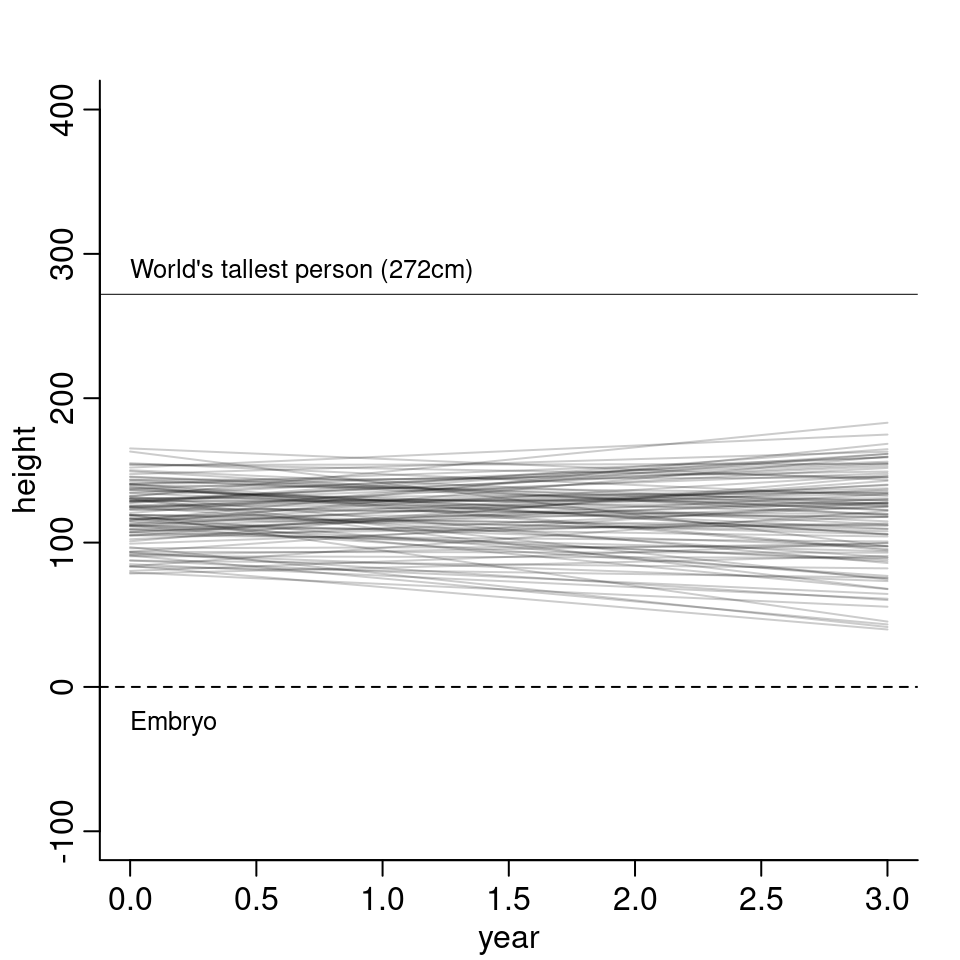
\includegraphics{chapter10a_files/figure-latex/unnamed-chunk-6-1}

Note also that the difference has a small standard error, so the order
of the models wouldn't easily change.

Let's have a look at the third model to understand why it performs
poorly compared with the second one:

\begin{Shaded}
\begin{Highlighting}[]
\KeywordTok{precis}\NormalTok{(m10}\FloatTok{.3}\NormalTok{)}
\end{Highlighting}
\end{Shaded}

\begin{verbatim}
     Mean StdDev  5.5% 94.5%
a    0.05   0.13 -0.15  0.25
bp   0.61   0.23  0.25  0.97
bpC -0.10   0.26 -0.53  0.32
\end{verbatim}

\begin{Shaded}
\begin{Highlighting}[]
\KeywordTok{plot}\NormalTok{(}\KeywordTok{precis}\NormalTok{(m10}\FloatTok{.3}\NormalTok{))}
\end{Highlighting}
\end{Shaded}

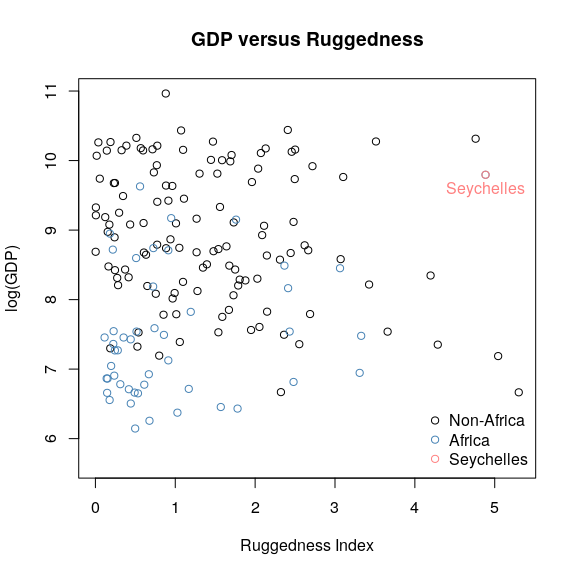
\includegraphics{chapter10a_files/figure-latex/unnamed-chunk-8-1}

The interaction variable has a rather wide posterior. Let's have a
closer look at the parameter \texttt{bp} for the effect of the prosocial
option. We have to distinguish between the absolute and relative effect.

Changing the predictor \texttt{prosoc\_left} from 0 to 1 increases the
log-odds of pulling the left-hand lever by 0.61. This implies the odds
are multiplied by:

\begin{Shaded}
\begin{Highlighting}[]
\KeywordTok{exp}\NormalTok{(}\FloatTok{0.61}\NormalTok{)}
\end{Highlighting}
\end{Shaded}

\begin{verbatim}
[1] 1.840431
\end{verbatim}

That is, the odds increase by 84\%. This is the relative effect. The
relative effect depend strongly on the other parameter als well. If we
assume for example an \(\alpha\) value of 4 then the probability for a
pull, ignoring everything else:

\begin{Shaded}
\begin{Highlighting}[]
\KeywordTok{logistic}\NormalTok{(}\DecValTok{4}\NormalTok{)}
\end{Highlighting}
\end{Shaded}

\begin{verbatim}
[1] 0.9820138
\end{verbatim}

is already quite high. Adding then the increase of 0.61 (relative
increase of 84\%) changes this to

\begin{Shaded}
\begin{Highlighting}[]
\KeywordTok{logistic}\NormalTok{(}\DecValTok{4} \OperatorTok{+}\StringTok{ }\FloatTok{0.61}\NormalTok{)}
\end{Highlighting}
\end{Shaded}

\begin{verbatim}
[1] 0.9901462
\end{verbatim}

In this example, the absolute effect would thus be small.

Let's plot the absolute effect:

\begin{Shaded}
\begin{Highlighting}[]
\CommentTok{# dummy data for predictions across treatments}
\NormalTok{d.pred <-}\StringTok{ }\KeywordTok{data.frame}\NormalTok{(}
  \DataTypeTok{prosoc_left =} \KeywordTok{c}\NormalTok{(}\DecValTok{0}\NormalTok{, }\DecValTok{1}\NormalTok{, }\DecValTok{0}\NormalTok{, }\DecValTok{1}\NormalTok{), }\CommentTok{# right/left/right/left}
  \DataTypeTok{condition =} \KeywordTok{c}\NormalTok{(}\DecValTok{0}\NormalTok{, }\DecValTok{0}\NormalTok{, }\DecValTok{1}\NormalTok{, }\DecValTok{1}\NormalTok{)    }\CommentTok{# control/control/partner/partner}
\NormalTok{)}

\CommentTok{# build prediction ensemble}
\NormalTok{chimp.ensemble <-}\StringTok{ }\KeywordTok{ensemble}\NormalTok{(m10}\FloatTok{.1}\NormalTok{, m10}\FloatTok{.2}\NormalTok{, m10}\FloatTok{.3}\NormalTok{, }\DataTypeTok{data=}\NormalTok{d.pred)}

\CommentTok{# summarize}
\NormalTok{pred.p <-}\StringTok{ }\KeywordTok{apply}\NormalTok{(chimp.ensemble}\OperatorTok{$}\NormalTok{link, }\DecValTok{2}\NormalTok{, mean)}
\NormalTok{pred.p.PI <-}\StringTok{ }\KeywordTok{apply}\NormalTok{(chimp.ensemble}\OperatorTok{$}\NormalTok{link, }\DecValTok{2}\NormalTok{, PI)}
\end{Highlighting}
\end{Shaded}

\begin{Shaded}
\begin{Highlighting}[]
\KeywordTok{plot}\NormalTok{(}\DecValTok{0}\NormalTok{, }\DecValTok{0}\NormalTok{, }\DataTypeTok{type =} \StringTok{"n"}\NormalTok{, }\DataTypeTok{xlab =} \StringTok{"prosoc_left/condition"}\NormalTok{, }
    \DataTypeTok{ylab =} \StringTok{"proportion pulled left"}\NormalTok{, }\DataTypeTok{ylim =} \KeywordTok{c}\NormalTok{(}\DecValTok{0}\NormalTok{, }
        \DecValTok{1}\NormalTok{), }\DataTypeTok{xaxt =} \StringTok{"n"}\NormalTok{, }\DataTypeTok{xlim =} \KeywordTok{c}\NormalTok{(}\DecValTok{1}\NormalTok{, }\DecValTok{4}\NormalTok{))}
\KeywordTok{axis}\NormalTok{(}\DecValTok{1}\NormalTok{, }\DataTypeTok{at =} \DecValTok{1}\OperatorTok{:}\DecValTok{4}\NormalTok{, }\DataTypeTok{labels =} \KeywordTok{c}\NormalTok{(}\StringTok{"0/0"}\NormalTok{, }\StringTok{"1/0"}\NormalTok{, }\StringTok{"0/1"}\NormalTok{, }
    \StringTok{"1/1"}\NormalTok{))}

\NormalTok{p <-}\StringTok{ }\KeywordTok{by}\NormalTok{(d}\OperatorTok{$}\NormalTok{pulled_left, }\KeywordTok{list}\NormalTok{(d}\OperatorTok{$}\NormalTok{prosoc_left, d}\OperatorTok{$}\NormalTok{condition, }
\NormalTok{    d}\OperatorTok{$}\NormalTok{actor), mean)}

\ControlFlowTok{for}\NormalTok{ (chimp }\ControlFlowTok{in} \DecValTok{1}\OperatorTok{:}\DecValTok{7}\NormalTok{) }\KeywordTok{lines}\NormalTok{(}\DecValTok{1}\OperatorTok{:}\DecValTok{4}\NormalTok{, }\KeywordTok{as.vector}\NormalTok{(p[, , }
\NormalTok{    chimp]), }\DataTypeTok{col =} \StringTok{"royalblue4"}\NormalTok{, }\DataTypeTok{lwd =} \FloatTok{1.5}\NormalTok{)}

\KeywordTok{lines}\NormalTok{(}\DecValTok{1}\OperatorTok{:}\DecValTok{4}\NormalTok{, pred.p)}
\KeywordTok{shade}\NormalTok{(pred.p.PI, }\DecValTok{1}\OperatorTok{:}\DecValTok{4}\NormalTok{)}
\end{Highlighting}
\end{Shaded}

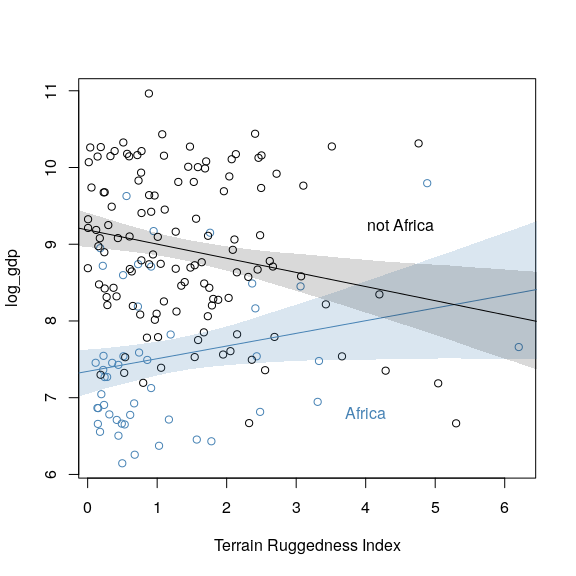
\includegraphics{chapter10a_files/figure-latex/unnamed-chunk-13-1}

Compare the MAP model with a MCMC Stan model:

\begin{Shaded}
\begin{Highlighting}[]
\CommentTok{# clean NAs from the data}
\NormalTok{d2 <-}\StringTok{ }\NormalTok{d}
\NormalTok{d2}\OperatorTok{$}\NormalTok{recipient <-}\StringTok{ }\OtherTok{NULL}

\CommentTok{# re-use map fit to get the formula}
\NormalTok{m10}\FloatTok{.3}\NormalTok{stan <-}\StringTok{ }\KeywordTok{map2stan}\NormalTok{(m10}\FloatTok{.3}\NormalTok{, }\DataTypeTok{data =}\NormalTok{ d2, }\DataTypeTok{iter =} \DecValTok{10000}\NormalTok{, }
    \DataTypeTok{warmup =} \DecValTok{1000}\NormalTok{)}
\KeywordTok{precis}\NormalTok{(m10}\FloatTok{.3}\NormalTok{stan)}
\end{Highlighting}
\end{Shaded}

\begin{Shaded}
\begin{Highlighting}[]
\KeywordTok{precis}\NormalTok{(m10}\FloatTok{.3}\NormalTok{stan)}
\end{Highlighting}
\end{Shaded}

\begin{verbatim}
     Mean StdDev lower 0.89 upper 0.89 n_eff
a    0.05   0.13      -0.16       0.24  4846
bp   0.61   0.22       0.27       0.98  4279
bpC -0.11   0.26      -0.55       0.30  5137
    Rhat
a      1
bp     1
bpC    1
\end{verbatim}

The numbers are almost identical with the MAP model and we can check the
pairs plot to see that the posterior is indeed well approximated by a
quadratic.

\begin{Shaded}
\begin{Highlighting}[]
\KeywordTok{pairs}\NormalTok{(m10}\FloatTok{.3}\NormalTok{stan)}
\end{Highlighting}
\end{Shaded}

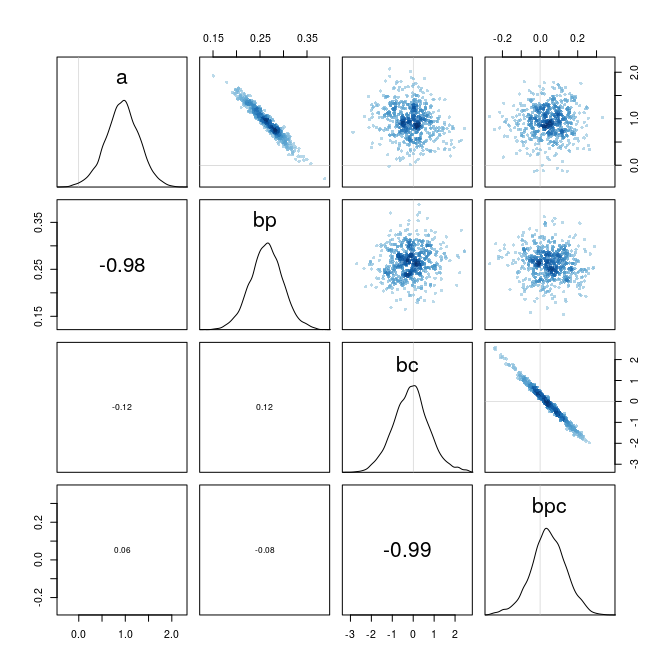
\includegraphics{chapter10a_files/figure-latex/unnamed-chunk-16-1}

We saw in the plot of the average proportions pulled left above that
some chimpanzees have a preference for pulling the left or right lever.
One even always pulled the left lever. A factor here might be the
handedness of the chimp. One thing we can do, is to fit an intercept for
each individula: \[\begin{align*}
L_i &\sim \text{Binomial}(1, p_i)\\
\text{logit}(p_i) &= \alpha_{\text{ACTOR}[i]} + (\beta_P + \beta_{PC}C_i)P_i \\
\alpha &\sim \text{Normal}(0, 10) \\
\beta_P &\sim \text{Normal}(0, 10) \\
\beta_{PC} &\sim \text{Normal}(0, 10) 
\end{align*}\] We fit this with MCMC since it will turn out to have some
skew in its posterior distribution.

\begin{Shaded}
\begin{Highlighting}[]
\NormalTok{m10}\FloatTok{.4}\NormalTok{ <-}\StringTok{ }\KeywordTok{map2stan}\NormalTok{(}\KeywordTok{alist}\NormalTok{(pulled_left }\OperatorTok{~}\StringTok{ }\KeywordTok{dbinom}\NormalTok{(}\DecValTok{1}\NormalTok{, }
\NormalTok{    p), }\KeywordTok{logit}\NormalTok{(p) <-}\StringTok{ }\NormalTok{a[actor] }\OperatorTok{+}\StringTok{ }\NormalTok{(bp }\OperatorTok{+}\StringTok{ }\NormalTok{bpC }\OperatorTok{*}\StringTok{ }\NormalTok{condition) }\OperatorTok{*}\StringTok{ }
\StringTok{    }\NormalTok{prosoc_left, a[actor] }\OperatorTok{~}\StringTok{ }\KeywordTok{dnorm}\NormalTok{(}\DecValTok{0}\NormalTok{, }\DecValTok{10}\NormalTok{), bp }\OperatorTok{~}\StringTok{ }
\StringTok{    }\KeywordTok{dnorm}\NormalTok{(}\DecValTok{0}\NormalTok{, }\DecValTok{10}\NormalTok{), bpC }\OperatorTok{~}\StringTok{ }\KeywordTok{dnorm}\NormalTok{(}\DecValTok{0}\NormalTok{, }\DecValTok{10}\NormalTok{)), }\DataTypeTok{data =}\NormalTok{ d2, }
    \DataTypeTok{chains =} \DecValTok{2}\NormalTok{, }\DataTypeTok{iter =} \DecValTok{2500}\NormalTok{, }\DataTypeTok{warmup =} \DecValTok{500}\NormalTok{)}
\end{Highlighting}
\end{Shaded}

Number of actors:

\begin{Shaded}
\begin{Highlighting}[]
\KeywordTok{unique}\NormalTok{(d}\OperatorTok{$}\NormalTok{actor)}
\end{Highlighting}
\end{Shaded}

\begin{verbatim}
[1] 1 2 3 4 5 6 7
\end{verbatim}

\begin{Shaded}
\begin{Highlighting}[]
\KeywordTok{precis}\NormalTok{(m10}\FloatTok{.4}\NormalTok{, }\DataTypeTok{depth =} \DecValTok{2}\NormalTok{)}
\end{Highlighting}
\end{Shaded}

\begin{verbatim}
      Mean StdDev lower 0.89 upper 0.89
a[1] -0.75   0.28      -1.19      -0.32
a[2] 11.08   5.47       3.55      18.78
a[3] -1.06   0.28      -1.48      -0.59
a[4] -1.06   0.28      -1.53      -0.64
a[5] -0.75   0.27      -1.21      -0.34
a[6]  0.22   0.27      -0.20       0.65
a[7]  1.81   0.39       1.24       2.45
bp    0.85   0.26       0.42       1.24
bpC  -0.14   0.29      -0.61       0.31
     n_eff Rhat
a[1]  3414    1
a[2]  1387    1
a[3]  3192    1
a[4]  3231    1
a[5]  3280    1
a[6]  3461    1
a[7]  4000    1
bp    2333    1
bpC   3135    1
\end{verbatim}

This posterior is not entirely Gaussian:

\begin{Shaded}
\begin{Highlighting}[]
\NormalTok{post <-}\StringTok{ }\KeywordTok{extract.samples}\NormalTok{(m10}\FloatTok{.4}\NormalTok{)}
\KeywordTok{str}\NormalTok{(post)}
\end{Highlighting}
\end{Shaded}

\begin{verbatim}
List of 3
 $ a  : num [1:4000, 1:7] -0.452 -0.402 -0.56 -0.511 -0.48 ...
 $ bp : num [1:4000(1d)] 0.751 0.684 0.917 0.762 0.718 ...
 $ bpC: num [1:4000(1d)] -0.0582 0.3174 -0.1897 -0.2928 -0.2148 ...
\end{verbatim}

\begin{Shaded}
\begin{Highlighting}[]
\KeywordTok{dens}\NormalTok{(post}\OperatorTok{$}\NormalTok{a[, }\DecValTok{2}\NormalTok{])}
\end{Highlighting}
\end{Shaded}

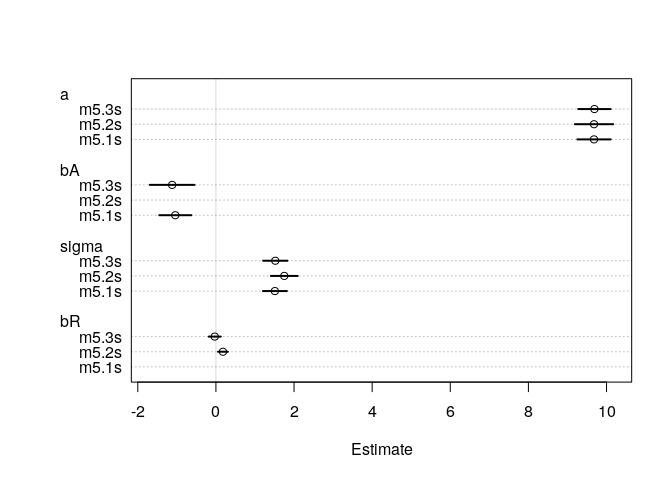
\includegraphics{chapter10a_files/figure-latex/unnamed-chunk-21-1}

Plotting the predictions for each actor:

\begin{Shaded}
\begin{Highlighting}[]
\KeywordTok{par}\NormalTok{(}\DataTypeTok{mfrow=}\KeywordTok{c}\NormalTok{(}\DecValTok{4}\NormalTok{, }\DecValTok{2}\NormalTok{))}
\ControlFlowTok{for}\NormalTok{ (chimp }\ControlFlowTok{in} \DecValTok{1}\OperatorTok{:}\DecValTok{7}\NormalTok{) \{}
\NormalTok{  d.pred <-}\StringTok{ }\KeywordTok{list}\NormalTok{(}
    \DataTypeTok{pulled_left =} \KeywordTok{rep}\NormalTok{(}\DecValTok{0}\NormalTok{, }\DecValTok{4}\NormalTok{),       }\CommentTok{# empty outcomes}
    \DataTypeTok{prosoc_left =} \KeywordTok{c}\NormalTok{(}\DecValTok{0}\NormalTok{, }\DecValTok{1}\NormalTok{, }\DecValTok{0}\NormalTok{, }\DecValTok{1}\NormalTok{),   }\CommentTok{# right/left/right/left}
    \DataTypeTok{condition =} \KeywordTok{c}\NormalTok{(}\DecValTok{0}\NormalTok{, }\DecValTok{0}\NormalTok{, }\DecValTok{1}\NormalTok{, }\DecValTok{1}\NormalTok{),     }\CommentTok{# control/control/partner/partner}
    \DataTypeTok{actor =} \KeywordTok{rep}\NormalTok{(chimp, }\DecValTok{4}\NormalTok{)}
\NormalTok{  )}
\NormalTok{  link.m10}\FloatTok{.4}\NormalTok{ <-}\StringTok{ }\KeywordTok{link}\NormalTok{( m10}\FloatTok{.4}\NormalTok{, }\DataTypeTok{data=}\NormalTok{d.pred)}
\NormalTok{  pred.p <-}\StringTok{ }\KeywordTok{apply}\NormalTok{( link.m10}\FloatTok{.4}\NormalTok{, }\DecValTok{2}\NormalTok{, mean)}
\NormalTok{  pred.p.PI <-}\StringTok{ }\KeywordTok{apply}\NormalTok{( link.m10}\FloatTok{.4}\NormalTok{, }\DecValTok{2}\NormalTok{, PI )}
  
  \KeywordTok{plot}\NormalTok{(}\DecValTok{0}\NormalTok{, }\DecValTok{0}\NormalTok{, }\DataTypeTok{type=}\StringTok{"n"}\NormalTok{, }\DataTypeTok{xlab=}\StringTok{"prosoc_left/condition"}\NormalTok{,}
       \DataTypeTok{ylab=}\StringTok{"proportion pulled left"}\NormalTok{,}
       \DataTypeTok{ylim=}\KeywordTok{c}\NormalTok{(}\DecValTok{0}\NormalTok{,}\DecValTok{1}\NormalTok{), }\DataTypeTok{xaxt=}\StringTok{"n"}\NormalTok{,}
       \DataTypeTok{xlim=}\KeywordTok{c}\NormalTok{(}\DecValTok{1}\NormalTok{, }\DecValTok{4}\NormalTok{), }\DataTypeTok{yaxp=}\KeywordTok{c}\NormalTok{(}\DecValTok{0}\NormalTok{,}\DecValTok{1}\NormalTok{,}\DecValTok{2}\NormalTok{) )}
  \KeywordTok{axis}\NormalTok{(}\DecValTok{1}\NormalTok{, }\DataTypeTok{at=}\DecValTok{1}\OperatorTok{:}\DecValTok{4}\NormalTok{, }\DataTypeTok{labels=}\KeywordTok{c}\NormalTok{(}\StringTok{"0/0"}\NormalTok{, }\StringTok{"1/0"}\NormalTok{, }\StringTok{"0/1"}\NormalTok{, }\StringTok{"1/1"}\NormalTok{))}
  \KeywordTok{mtext}\NormalTok{(}\KeywordTok{paste}\NormalTok{( }\StringTok{"actor"}\NormalTok{, chimp ))}
  
\NormalTok{  p <-}\StringTok{ }\KeywordTok{by}\NormalTok{( d}\OperatorTok{$}\NormalTok{pulled_left,}
           \KeywordTok{list}\NormalTok{(d}\OperatorTok{$}\NormalTok{prosoc_left, d}\OperatorTok{$}\NormalTok{condition, d}\OperatorTok{$}\NormalTok{actor), mean )}
  \KeywordTok{lines}\NormalTok{( }\DecValTok{1}\OperatorTok{:}\DecValTok{4}\NormalTok{, }\KeywordTok{as.vector}\NormalTok{(p[,,chimp]), }\DataTypeTok{col=}\StringTok{"royalblue4"}\NormalTok{, }\DataTypeTok{lwd=}\DecValTok{2}\NormalTok{)}
  
  \KeywordTok{lines}\NormalTok{(}\DecValTok{1}\OperatorTok{:}\DecValTok{4}\NormalTok{, pred.p)}
  \KeywordTok{shade}\NormalTok{(pred.p.PI, }\DecValTok{1}\OperatorTok{:}\DecValTok{4}\NormalTok{)}
\NormalTok{\}}
\end{Highlighting}
\end{Shaded}

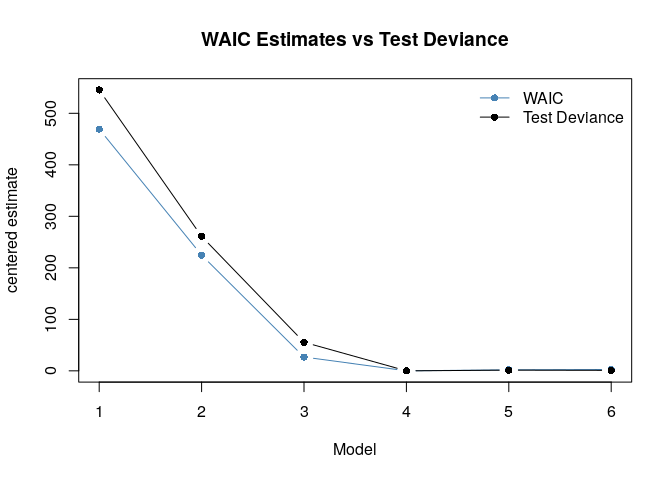
\includegraphics{chapter10a_files/figure-latex/unnamed-chunk-22-1}

\subsection{Aggregated binomial}\label{aggregated-binomial}

\subsubsection{Chimpanzees}\label{chimpanzees}

Instead of predicting the likelihood for a single pull (0 or 1), we can
also predict the counts, i.e.~how likely is it that an actor pulls left
\texttt{x} times out of 18 trials.

\begin{Shaded}
\begin{Highlighting}[]
\KeywordTok{data}\NormalTok{(chimpanzees)}
\NormalTok{d <-}\StringTok{ }\NormalTok{chimpanzees}
\NormalTok{d.aggregated <-}\StringTok{ }\KeywordTok{aggregate}\NormalTok{(d}\OperatorTok{$}\NormalTok{pulled_left, }\KeywordTok{list}\NormalTok{(}\DataTypeTok{prosoc_left =}\NormalTok{ d}\OperatorTok{$}\NormalTok{prosoc_left, }
    \DataTypeTok{condition =}\NormalTok{ d}\OperatorTok{$}\NormalTok{condition, }\DataTypeTok{actor =}\NormalTok{ d}\OperatorTok{$}\NormalTok{actor), }
\NormalTok{    sum)}
\NormalTok{knitr}\OperatorTok{::}\KeywordTok{kable}\NormalTok{(}\KeywordTok{head}\NormalTok{(d.aggregated, }\DecValTok{8}\NormalTok{))}
\end{Highlighting}
\end{Shaded}

\begin{longtable}[]{@{}rrrr@{}}
\toprule
prosoc\_left & condition & actor & x\tabularnewline
\midrule
\endhead
0 & 0 & 1 & 6\tabularnewline
1 & 0 & 1 & 9\tabularnewline
0 & 1 & 1 & 5\tabularnewline
1 & 1 & 1 & 10\tabularnewline
0 & 0 & 2 & 18\tabularnewline
1 & 0 & 2 & 18\tabularnewline
0 & 1 & 2 & 18\tabularnewline
1 & 1 & 2 & 18\tabularnewline
\bottomrule
\end{longtable}

\begin{Shaded}
\begin{Highlighting}[]
\NormalTok{m10}\FloatTok{.5}\NormalTok{ <-}\StringTok{ }\KeywordTok{map}\NormalTok{(}\KeywordTok{alist}\NormalTok{(x }\OperatorTok{~}\StringTok{ }\KeywordTok{dbinom}\NormalTok{(}\DecValTok{18}\NormalTok{, p), }\KeywordTok{logit}\NormalTok{(p) <-}\StringTok{ }\NormalTok{a }\OperatorTok{+}\StringTok{ }
\StringTok{    }\NormalTok{(bp }\OperatorTok{+}\StringTok{ }\NormalTok{bpC }\OperatorTok{*}\StringTok{ }\NormalTok{condition) }\OperatorTok{*}\StringTok{ }\NormalTok{prosoc_left, a }\OperatorTok{~}\StringTok{ }
\StringTok{    }\KeywordTok{dnorm}\NormalTok{(}\DecValTok{0}\NormalTok{, }\DecValTok{10}\NormalTok{), bp }\OperatorTok{~}\StringTok{ }\KeywordTok{dnorm}\NormalTok{(}\DecValTok{0}\NormalTok{, }\DecValTok{10}\NormalTok{), bpC }\OperatorTok{~}\StringTok{ }\KeywordTok{dnorm}\NormalTok{(}\DecValTok{0}\NormalTok{, }
    \DecValTok{10}\NormalTok{)), }\DataTypeTok{data =}\NormalTok{ d.aggregated)}
\KeywordTok{precis}\NormalTok{(m10}\FloatTok{.5}\NormalTok{)}
\end{Highlighting}
\end{Shaded}

\begin{verbatim}
     Mean StdDev  5.5% 94.5%
a    0.05   0.13 -0.15  0.25
bp   0.61   0.23  0.25  0.97
bpC -0.10   0.26 -0.53  0.32
\end{verbatim}

Compare with the same model with non-aggregated data:

\begin{Shaded}
\begin{Highlighting}[]
\KeywordTok{precis}\NormalTok{(m10}\FloatTok{.3}\NormalTok{stan)}
\end{Highlighting}
\end{Shaded}

\begin{verbatim}
     Mean StdDev lower 0.89 upper 0.89 n_eff
a    0.05   0.13      -0.16       0.24  4846
bp   0.61   0.22       0.27       0.98  4279
bpC -0.11   0.26      -0.55       0.30  5137
    Rhat
a      1
bp     1
bpC    1
\end{verbatim}

We get the same estimates.

\subsubsection{Graduate school
admissions}\label{graduate-school-admissions}

\begin{Shaded}
\begin{Highlighting}[]
\KeywordTok{data}\NormalTok{(}\StringTok{"UCBadmit"}\NormalTok{)}
\NormalTok{d <-}\StringTok{ }\NormalTok{UCBadmit}
\NormalTok{knitr}\OperatorTok{::}\KeywordTok{kable}\NormalTok{(d)}
\end{Highlighting}
\end{Shaded}

\begin{longtable}[]{@{}llrrr@{}}
\toprule
dept & applicant.gender & admit & reject & applications\tabularnewline
\midrule
\endhead
A & male & 512 & 313 & 825\tabularnewline
A & female & 89 & 19 & 108\tabularnewline
B & male & 353 & 207 & 560\tabularnewline
B & female & 17 & 8 & 25\tabularnewline
C & male & 120 & 205 & 325\tabularnewline
C & female & 202 & 391 & 593\tabularnewline
D & male & 138 & 279 & 417\tabularnewline
D & female & 131 & 244 & 375\tabularnewline
E & male & 53 & 138 & 191\tabularnewline
E & female & 94 & 299 & 393\tabularnewline
F & male & 22 & 351 & 373\tabularnewline
F & female & 24 & 317 & 341\tabularnewline
\bottomrule
\end{longtable}

The data set contains only 12 rows but since it is aggregated, it
actually represents 4526 applications. The goal is to evaluate whether
the data contains evidence for gender bias in admission.

We will fit two models: One using gender as a predictor for
\texttt{admit} and one modelling \texttt{admit} as a constant, ignoring
gender.

\begin{Shaded}
\begin{Highlighting}[]
\NormalTok{d}\OperatorTok{$}\NormalTok{male <-}\StringTok{ }\KeywordTok{ifelse}\NormalTok{(d}\OperatorTok{$}\NormalTok{applicant.gender }\OperatorTok{==}\StringTok{ "male"}\NormalTok{, }
    \DecValTok{1}\NormalTok{, }\DecValTok{0}\NormalTok{)}

\NormalTok{m10}\FloatTok{.6}\NormalTok{ <-}\StringTok{ }\KeywordTok{map}\NormalTok{(}\KeywordTok{alist}\NormalTok{(admit }\OperatorTok{~}\StringTok{ }\KeywordTok{dbinom}\NormalTok{(applications, }
\NormalTok{    p), }\KeywordTok{logit}\NormalTok{(p) <-}\StringTok{ }\NormalTok{a }\OperatorTok{+}\StringTok{ }\NormalTok{bm }\OperatorTok{*}\StringTok{ }\NormalTok{male, a }\OperatorTok{~}\StringTok{ }\KeywordTok{dnorm}\NormalTok{(}\DecValTok{0}\NormalTok{, }
    \DecValTok{10}\NormalTok{), bm }\OperatorTok{~}\StringTok{ }\KeywordTok{dnorm}\NormalTok{(}\DecValTok{0}\NormalTok{, }\DecValTok{10}\NormalTok{)), }\DataTypeTok{data =}\NormalTok{ d)}

\NormalTok{m10}\FloatTok{.7}\NormalTok{ <-}\StringTok{ }\KeywordTok{map}\NormalTok{(}\KeywordTok{alist}\NormalTok{(admit }\OperatorTok{~}\StringTok{ }\KeywordTok{dbinom}\NormalTok{(applications, }
\NormalTok{    p), }\KeywordTok{logit}\NormalTok{(p) <-}\StringTok{ }\NormalTok{a, a }\OperatorTok{~}\StringTok{ }\KeywordTok{dnorm}\NormalTok{(}\DecValTok{0}\NormalTok{, }\DecValTok{10}\NormalTok{)), }\DataTypeTok{data =}\NormalTok{ d)}
\end{Highlighting}
\end{Shaded}

\begin{Shaded}
\begin{Highlighting}[]
\NormalTok{(cp <-}\StringTok{ }\KeywordTok{compare}\NormalTok{(m10}\FloatTok{.6}\NormalTok{, m10}\FloatTok{.7}\NormalTok{))}
\end{Highlighting}
\end{Shaded}

\begin{verbatim}
        WAIC pWAIC dWAIC weight    SE  dSE
m10.6 5954.7   1.9   0.0      1 35.00   NA
m10.7 6046.6   1.1  91.9      0 29.96 19.2
\end{verbatim}

The model using male as a predictor performs better than without. The
comparison suggests that gender actually matters a lot:

\begin{Shaded}
\begin{Highlighting}[]
\KeywordTok{plot}\NormalTok{(cp, }\DataTypeTok{xlim =} \KeywordTok{c}\NormalTok{(}\KeywordTok{min}\NormalTok{(cp}\OperatorTok{@}\NormalTok{output}\OperatorTok{$}\NormalTok{WAIC }\OperatorTok{-}\StringTok{ }\NormalTok{cp}\OperatorTok{@}\NormalTok{output}\OperatorTok{$}\NormalTok{SE), }
    \KeywordTok{max}\NormalTok{(cp}\OperatorTok{@}\NormalTok{output}\OperatorTok{$}\NormalTok{WAIC }\OperatorTok{+}\StringTok{ }\NormalTok{cp}\OperatorTok{@}\NormalTok{output}\OperatorTok{$}\NormalTok{SE)))}
\end{Highlighting}
\end{Shaded}

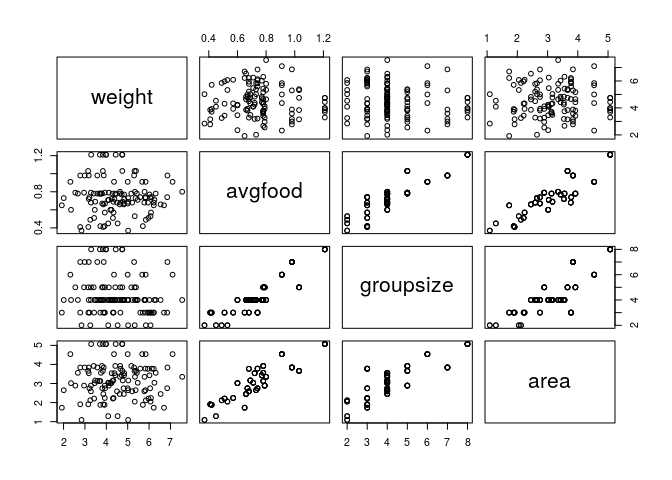
\includegraphics{chapter10a_files/figure-latex/unnamed-chunk-29-1}

In which way does it matter?

\begin{Shaded}
\begin{Highlighting}[]
\KeywordTok{precis}\NormalTok{(m10}\FloatTok{.6}\NormalTok{)}
\end{Highlighting}
\end{Shaded}

\begin{verbatim}
    Mean StdDev  5.5% 94.5%
a  -0.83   0.05 -0.91 -0.75
bm  0.61   0.06  0.51  0.71
\end{verbatim}

Being male does improve the chances of being admitted. The relative
difference is \texttt{exp(0.61)\ =} 1.8404314. This means that a male
applicant's odds are 184\% of a female applicant. Let's get the absolute
scale, which is more important:

\begin{Shaded}
\begin{Highlighting}[]
\NormalTok{post <-}\StringTok{ }\KeywordTok{extract.samples}\NormalTok{(m10}\FloatTok{.6}\NormalTok{)}
\NormalTok{p.admit.male <-}\StringTok{ }\KeywordTok{logistic}\NormalTok{(post}\OperatorTok{$}\NormalTok{a }\OperatorTok{+}\StringTok{ }\NormalTok{post}\OperatorTok{$}\NormalTok{bm)}
\NormalTok{p.admit.female <-}\StringTok{ }\KeywordTok{logistic}\NormalTok{(post}\OperatorTok{$}\NormalTok{a)}

\NormalTok{diff.admit <-}\StringTok{ }\NormalTok{p.admit.male }\OperatorTok{-}\StringTok{ }\NormalTok{p.admit.female}

\KeywordTok{quantile}\NormalTok{(diff.admit, }\KeywordTok{c}\NormalTok{(}\FloatTok{0.025}\NormalTok{, }\FloatTok{0.5}\NormalTok{, }\FloatTok{0.975}\NormalTok{))}
\end{Highlighting}
\end{Shaded}

\begin{verbatim}
     2.5%       50%     97.5% 
0.1130201 0.1413141 0.1692898 
\end{verbatim}

Thus the median estimate of the male advantage is about 14\%.

\begin{Shaded}
\begin{Highlighting}[]
\KeywordTok{dens}\NormalTok{(diff.admit)}
\end{Highlighting}
\end{Shaded}

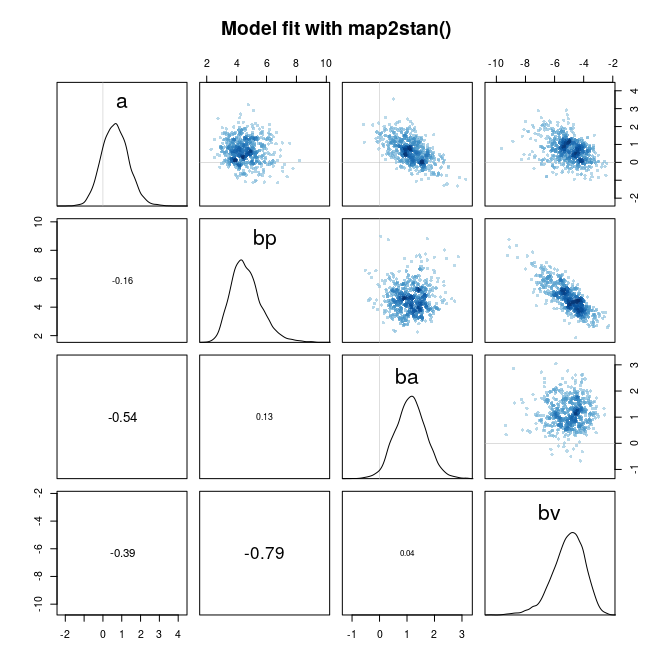
\includegraphics{chapter10a_files/figure-latex/unnamed-chunk-32-1}

\begin{Shaded}
\begin{Highlighting}[]
\KeywordTok{postcheck}\NormalTok{(m10}\FloatTok{.6}\NormalTok{, }\DataTypeTok{n =} \DecValTok{10000}\NormalTok{, }\DataTypeTok{col =} \StringTok{"royalblue4"}\NormalTok{)}

\CommentTok{# draw lines connecting points from same dept}
\ControlFlowTok{for}\NormalTok{ (i }\ControlFlowTok{in} \DecValTok{1}\OperatorTok{:}\DecValTok{6}\NormalTok{) \{}
\NormalTok{    x <-}\StringTok{ }\DecValTok{1} \OperatorTok{+}\StringTok{ }\DecValTok{2} \OperatorTok{*}\StringTok{ }\NormalTok{(i }\OperatorTok{-}\StringTok{ }\DecValTok{1}\NormalTok{)}
\NormalTok{    y1 <-}\StringTok{ }\NormalTok{d}\OperatorTok{$}\NormalTok{admit[x]}\OperatorTok{/}\NormalTok{d}\OperatorTok{$}\NormalTok{applications[x]  }\CommentTok{# male}
\NormalTok{    y2 <-}\StringTok{ }\NormalTok{d}\OperatorTok{$}\NormalTok{admit[x }\OperatorTok{+}\StringTok{ }\DecValTok{1}\NormalTok{]}\OperatorTok{/}\NormalTok{d}\OperatorTok{$}\NormalTok{applications[x }\OperatorTok{+}\StringTok{ }\DecValTok{1}\NormalTok{]  }\CommentTok{# female}
    \KeywordTok{lines}\NormalTok{(}\KeywordTok{c}\NormalTok{(x, x }\OperatorTok{+}\StringTok{ }\DecValTok{1}\NormalTok{), }\KeywordTok{c}\NormalTok{(y1, y2), }\DataTypeTok{col =} \StringTok{"royalblue4"}\NormalTok{, }
        \DataTypeTok{lwd =} \DecValTok{2}\NormalTok{)}
    \KeywordTok{text}\NormalTok{(x }\OperatorTok{+}\StringTok{ }\FloatTok{0.5}\NormalTok{, (y1 }\OperatorTok{+}\StringTok{ }\NormalTok{y2)}\OperatorTok{/}\DecValTok{2} \OperatorTok{+}\StringTok{ }\FloatTok{0.05}\NormalTok{, d}\OperatorTok{$}\NormalTok{dept[x], }
        \DataTypeTok{cex =} \FloatTok{0.8}\NormalTok{, }\DataTypeTok{col =} \StringTok{"royalblue4"}\NormalTok{)}
\NormalTok{\}}
\end{Highlighting}
\end{Shaded}

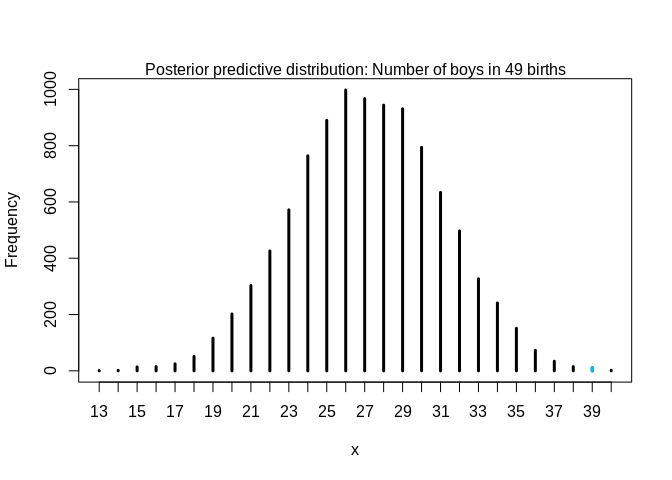
\includegraphics{chapter10a_files/figure-latex/unnamed-chunk-33-1}

The first point of a line is the admission rate for males while the
second point of a line is the admission rate for females. The expeted
predictions are the black open points and the black crosses indicate the
89\% interval of the expectations. The plot shows that only two
departments (C and E) and lower admission rates for females. How come we
get such a bad prediction?

The problem: Male and female applicants don't apply to the same
departments and departments have different admission rates. Department A
has much higer admission rates than department F and female applicants
apply more often to F than to A.

We will build a model that uses a unique intercept per department.

\begin{Shaded}
\begin{Highlighting}[]
\CommentTok{# make index}
\NormalTok{d}\OperatorTok{$}\NormalTok{dept_id <-}\StringTok{ }\KeywordTok{coerce_index}\NormalTok{(d}\OperatorTok{$}\NormalTok{dept)}

\CommentTok{# model with unique intercept for each dept}
\NormalTok{m10}\FloatTok{.8}\NormalTok{ <-}\StringTok{ }\KeywordTok{map}\NormalTok{(}\KeywordTok{alist}\NormalTok{(admit }\OperatorTok{~}\StringTok{ }\KeywordTok{dbinom}\NormalTok{(applications, }
\NormalTok{    p), }\KeywordTok{logit}\NormalTok{(p) <-}\StringTok{ }\NormalTok{a[dept_id], a[dept_id] }\OperatorTok{~}\StringTok{ }\KeywordTok{dnorm}\NormalTok{(}\DecValTok{0}\NormalTok{, }
    \DecValTok{10}\NormalTok{)), }\DataTypeTok{data =}\NormalTok{ d)}

\NormalTok{m10}\FloatTok{.9}\NormalTok{ <-}\StringTok{ }\KeywordTok{map}\NormalTok{(}\KeywordTok{alist}\NormalTok{(admit }\OperatorTok{~}\StringTok{ }\KeywordTok{dbinom}\NormalTok{(applications, }
\NormalTok{    p), }\KeywordTok{logit}\NormalTok{(p) <-}\StringTok{ }\NormalTok{a[dept_id] }\OperatorTok{+}\StringTok{ }\NormalTok{bm }\OperatorTok{*}\StringTok{ }\NormalTok{male, a[dept_id] }\OperatorTok{~}\StringTok{ }
\StringTok{    }\KeywordTok{dnorm}\NormalTok{(}\DecValTok{0}\NormalTok{, }\DecValTok{10}\NormalTok{), bm }\OperatorTok{~}\StringTok{ }\KeywordTok{dnorm}\NormalTok{(}\DecValTok{0}\NormalTok{, }\DecValTok{10}\NormalTok{)), }\DataTypeTok{data =}\NormalTok{ d)}
\end{Highlighting}
\end{Shaded}

We then compare all three models:

\begin{Shaded}
\begin{Highlighting}[]
\NormalTok{(cp <-}\StringTok{ }\KeywordTok{compare}\NormalTok{(m10}\FloatTok{.6}\NormalTok{, m10}\FloatTok{.7}\NormalTok{, m10}\FloatTok{.8}\NormalTok{, m10}\FloatTok{.9}\NormalTok{))}
\end{Highlighting}
\end{Shaded}

\begin{verbatim}
        WAIC pWAIC dWAIC weight    SE   dSE
m10.8 5201.1     6   0.0   0.55 57.04    NA
m10.9 5201.5     7   0.4   0.45 57.19  2.49
m10.6 5954.9     2 753.8   0.00 35.12 48.51
m10.7 6046.3     1 845.2   0.00 29.92 52.34
\end{verbatim}

As a plot:

\begin{Shaded}
\begin{Highlighting}[]
\KeywordTok{plot}\NormalTok{(cp, }\DataTypeTok{xlim =} \KeywordTok{c}\NormalTok{(}\KeywordTok{min}\NormalTok{(cp}\OperatorTok{@}\NormalTok{output}\OperatorTok{$}\NormalTok{WAIC }\OperatorTok{-}\StringTok{ }\NormalTok{cp}\OperatorTok{@}\NormalTok{output}\OperatorTok{$}\NormalTok{SE), }
    \KeywordTok{max}\NormalTok{(cp}\OperatorTok{@}\NormalTok{output}\OperatorTok{$}\NormalTok{WAIC }\OperatorTok{+}\StringTok{ }\NormalTok{cp}\OperatorTok{@}\NormalTok{output}\OperatorTok{$}\NormalTok{SE)))}
\end{Highlighting}
\end{Shaded}

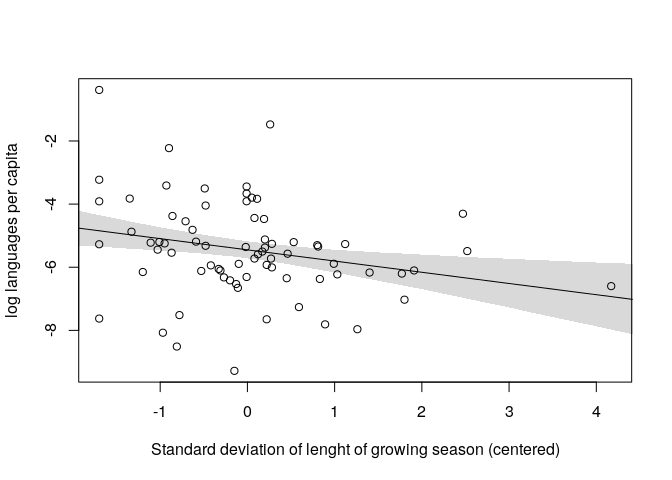
\includegraphics{chapter10a_files/figure-latex/unnamed-chunk-36-1}

The two new models with the unique intercepts perform much better. Now,
the model without \texttt{male} is ranked first but the difference
between the first two models is tiny. Both models got about half the
Akaike weight so you could call it a tie.

So how does gender now affect admission?

\begin{Shaded}
\begin{Highlighting}[]
\KeywordTok{precis}\NormalTok{(m10}\FloatTok{.9}\NormalTok{, }\DataTypeTok{depth =} \DecValTok{2}\NormalTok{)}
\end{Highlighting}
\end{Shaded}

\begin{verbatim}
      Mean StdDev  5.5% 94.5%
a[1]  0.68   0.10  0.52  0.84
a[2]  0.64   0.12  0.45  0.82
a[3] -0.58   0.07 -0.70 -0.46
a[4] -0.61   0.09 -0.75 -0.48
a[5] -1.06   0.10 -1.22 -0.90
a[6] -2.62   0.16 -2.88 -2.37
bm   -0.10   0.08 -0.23  0.03
\end{verbatim}

The estimate for \texttt{bm} has changed direction, meaning it now
estimates that being male is a disadvantage! The estimate becomes
\texttt{exp(-0.1)\ =} 0.9048374. So a male has about 90\% the odds of
admission as a female.

Let's do the posterior check again as before:

\begin{Shaded}
\begin{Highlighting}[]
\KeywordTok{postcheck}\NormalTok{(m10}\FloatTok{.9}\NormalTok{, }\DataTypeTok{n =} \DecValTok{10000}\NormalTok{, }\DataTypeTok{col =} \StringTok{"royalblue4"}\NormalTok{)}

\CommentTok{# draw lines connecting points from same dept}
\ControlFlowTok{for}\NormalTok{ (i }\ControlFlowTok{in} \DecValTok{1}\OperatorTok{:}\DecValTok{6}\NormalTok{) \{}
\NormalTok{    x <-}\StringTok{ }\DecValTok{1} \OperatorTok{+}\StringTok{ }\DecValTok{2} \OperatorTok{*}\StringTok{ }\NormalTok{(i }\OperatorTok{-}\StringTok{ }\DecValTok{1}\NormalTok{)}
\NormalTok{    y1 <-}\StringTok{ }\NormalTok{d}\OperatorTok{$}\NormalTok{admit[x]}\OperatorTok{/}\NormalTok{d}\OperatorTok{$}\NormalTok{applications[x]  }\CommentTok{# male}
\NormalTok{    y2 <-}\StringTok{ }\NormalTok{d}\OperatorTok{$}\NormalTok{admit[x }\OperatorTok{+}\StringTok{ }\DecValTok{1}\NormalTok{]}\OperatorTok{/}\NormalTok{d}\OperatorTok{$}\NormalTok{applications[x }\OperatorTok{+}\StringTok{ }\DecValTok{1}\NormalTok{]  }\CommentTok{# female}
    \KeywordTok{lines}\NormalTok{(}\KeywordTok{c}\NormalTok{(x, x }\OperatorTok{+}\StringTok{ }\DecValTok{1}\NormalTok{), }\KeywordTok{c}\NormalTok{(y1, y2), }\DataTypeTok{col =} \StringTok{"royalblue4"}\NormalTok{, }
        \DataTypeTok{lwd =} \DecValTok{2}\NormalTok{)}
    \KeywordTok{text}\NormalTok{(x }\OperatorTok{+}\StringTok{ }\FloatTok{0.5}\NormalTok{, (y1 }\OperatorTok{+}\StringTok{ }\NormalTok{y2)}\OperatorTok{/}\DecValTok{2} \OperatorTok{+}\StringTok{ }\FloatTok{0.05}\NormalTok{, d}\OperatorTok{$}\NormalTok{dept[x], }
        \DataTypeTok{cex =} \FloatTok{0.8}\NormalTok{, }\DataTypeTok{col =} \StringTok{"royalblue4"}\NormalTok{)}
\NormalTok{\}}
\end{Highlighting}
\end{Shaded}

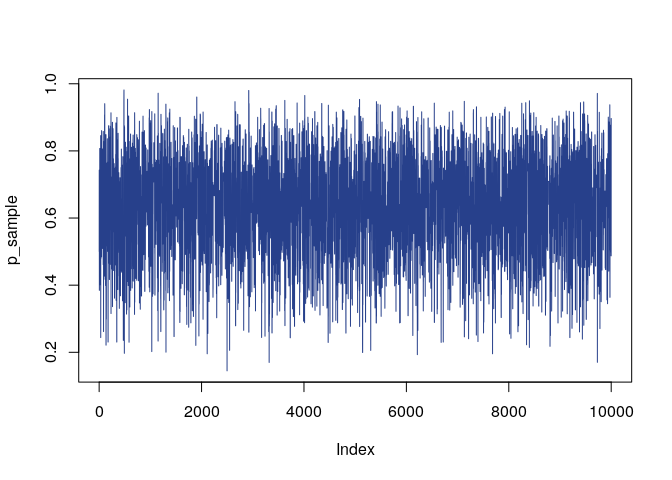
\includegraphics{chapter10a_files/figure-latex/unnamed-chunk-38-1}

The predictions fit much better than before.

Let's also check the quadratic approximation. In the example with the
chimpanzees, unique intercepts were a problem for quadratic
approximations, so let's check how the compare to a Stan model:

\begin{Shaded}
\begin{Highlighting}[]
\NormalTok{dstan <-}\StringTok{ }\NormalTok{d[, }\KeywordTok{c}\NormalTok{(}\StringTok{"admit"}\NormalTok{, }\StringTok{"applications"}\NormalTok{, }\StringTok{"male"}\NormalTok{, }
    \StringTok{"dept_id"}\NormalTok{)]}
\NormalTok{m10}\FloatTok{.9}\NormalTok{stan <-}\StringTok{ }\KeywordTok{map2stan}\NormalTok{(m10}\FloatTok{.9}\NormalTok{, }\DataTypeTok{data =}\NormalTok{ dstan, }\DataTypeTok{chains =} \DecValTok{2}\NormalTok{, }
    \DataTypeTok{iter =} \DecValTok{2500}\NormalTok{, }\DataTypeTok{warmup =} \DecValTok{500}\NormalTok{)}
\KeywordTok{precis}\NormalTok{(m10}\FloatTok{.9}\NormalTok{stan, }\DataTypeTok{depth =} \DecValTok{2}\NormalTok{)}
\end{Highlighting}
\end{Shaded}

\begin{Shaded}
\begin{Highlighting}[]
\KeywordTok{pairs}\NormalTok{(m10}\FloatTok{.9}\NormalTok{stan)}
\end{Highlighting}
\end{Shaded}

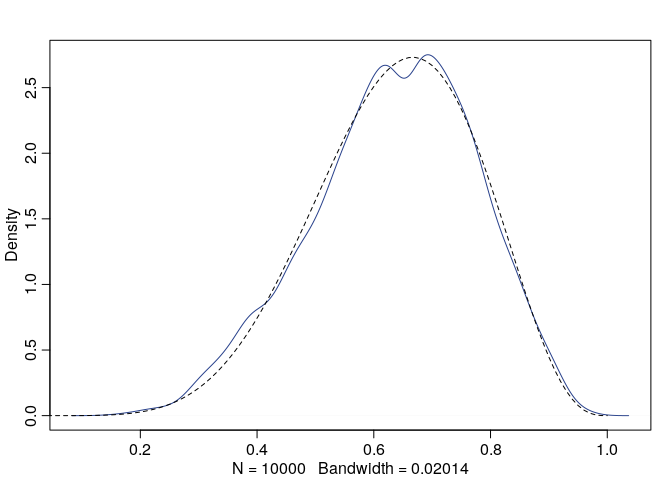
\includegraphics{chapter10a_files/figure-latex/unnamed-chunk-40-1}

All the posterior distributions are pretty much Gaussian, a quadratic
approximation thus gives good estimates.

\subsection{\texorpdfstring{Fitting binomial regression with
\texttt{glm}}{Fitting binomial regression with glm}}\label{fitting-binomial-regression-with-glm}

The following code yields similar results as the map approach for the
aggregated binomial.

\begin{Shaded}
\begin{Highlighting}[]
\NormalTok{m10}\FloatTok{.7}\NormalTok{glm <-}\StringTok{ }\KeywordTok{glm}\NormalTok{(}\KeywordTok{cbind}\NormalTok{(admit, reject) }\OperatorTok{~}\StringTok{ }\DecValTok{1}\NormalTok{, }\DataTypeTok{data =}\NormalTok{ d, }
    \DataTypeTok{family =}\NormalTok{ binomial)}
\NormalTok{m10}\FloatTok{.6}\NormalTok{glm <-}\StringTok{ }\KeywordTok{glm}\NormalTok{(}\KeywordTok{cbind}\NormalTok{(admit, reject) }\OperatorTok{~}\StringTok{ }\NormalTok{male, }\DataTypeTok{data =}\NormalTok{ d, }
    \DataTypeTok{family =}\NormalTok{ binomial)}
\NormalTok{m10}\FloatTok{.8}\NormalTok{glm <-}\StringTok{ }\KeywordTok{glm}\NormalTok{(}\KeywordTok{cbind}\NormalTok{(admit, reject) }\OperatorTok{~}\StringTok{ }\NormalTok{dept, }\DataTypeTok{data =}\NormalTok{ d, }
    \DataTypeTok{family =}\NormalTok{ binomial)}
\NormalTok{m10}\FloatTok{.9}\NormalTok{glm <-}\StringTok{ }\KeywordTok{glm}\NormalTok{(}\KeywordTok{cbind}\NormalTok{(admit, reject) }\OperatorTok{~}\StringTok{ }\NormalTok{male }\OperatorTok{+}\StringTok{ }
\StringTok{    }\NormalTok{dept, }\DataTypeTok{data =}\NormalTok{ d, }\DataTypeTok{family =}\NormalTok{ binomial)}
\KeywordTok{precis}\NormalTok{(m10}\FloatTok{.9}\NormalTok{glm)}
\end{Highlighting}
\end{Shaded}

\begin{verbatim}
             Mean StdDev  5.5% 94.5%
(Intercept)  0.68   0.10  0.52  0.84
male        -0.10   0.08 -0.23  0.03
deptB       -0.04   0.11 -0.22  0.13
deptC       -1.26   0.11 -1.43 -1.09
deptD       -1.29   0.11 -1.46 -1.13
deptE       -1.74   0.13 -1.94 -1.54
deptF       -3.31   0.17 -3.58 -3.03
\end{verbatim}

Compare with the \texttt{map()} model:

\begin{Shaded}
\begin{Highlighting}[]
\KeywordTok{precis}\NormalTok{(m10}\FloatTok{.9}\NormalTok{stan, }\DataTypeTok{depth =} \DecValTok{2}\NormalTok{)}
\end{Highlighting}
\end{Shaded}

\begin{verbatim}
      Mean StdDev lower 0.89 upper 0.89
a[1]  0.68   0.10       0.52       0.83
a[2]  0.64   0.11       0.45       0.82
a[3] -0.58   0.07      -0.70      -0.46
a[4] -0.61   0.09      -0.75      -0.48
a[5] -1.06   0.10      -1.21      -0.89
a[6] -2.63   0.16      -2.87      -2.37
bm   -0.10   0.08      -0.23       0.03
     n_eff Rhat
a[1]  2230    1
a[2]  2149    1
a[3]  3393    1
a[4]  3015    1
a[5]  4000    1
a[6]  4000    1
bm    1739    1
\end{verbatim}

Note that the departments are coded differently: the intercept in the
\texttt{glm} model corresponds to \texttt{a{[}1{]}} in the Stan model
and \texttt{deptB} in the \texttt{glm} model corresponds to the
difference from department A to B, that is \texttt{a{[}2{]}-a{[}1{]}} in
the Stan model.

To use \texttt{glm()} for a non-aggregated model:

\begin{Shaded}
\begin{Highlighting}[]
\NormalTok{m10}\FloatTok{.4}\NormalTok{glm <-}\StringTok{ }\KeywordTok{glm}\NormalTok{(pulled_left }\OperatorTok{~}\StringTok{ }\KeywordTok{as.factor}\NormalTok{(actor) }\OperatorTok{+}\StringTok{ }
\StringTok{    }\NormalTok{prosoc_left }\OperatorTok{*}\StringTok{ }\NormalTok{condition }\OperatorTok{-}\StringTok{ }\NormalTok{condition, }\DataTypeTok{data =}\NormalTok{ chimpanzees, }
    \DataTypeTok{family =}\NormalTok{ binomial)}
\KeywordTok{precis}\NormalTok{(m10}\FloatTok{.4}\NormalTok{glm)}
\end{Highlighting}
\end{Shaded}

\begin{verbatim}
                       Mean StdDev     5.5%
(Intercept)           -0.73   0.27    -1.16
as.factor(actor)2     18.95 754.98 -1187.65
as.factor(actor)3     -0.30   0.35    -0.86
as.factor(actor)4     -0.30   0.35    -0.86
as.factor(actor)5      0.00   0.34    -0.55
as.factor(actor)6      0.94   0.35     0.38
as.factor(actor)7      2.48   0.45     1.76
prosoc_left            0.82   0.26     0.40
prosoc_left:condition -0.13   0.30    -0.61
                        94.5%
(Intercept)             -0.30
as.factor(actor)2     1225.55
as.factor(actor)3        0.25
as.factor(actor)4        0.25
as.factor(actor)5        0.55
as.factor(actor)6        1.50
as.factor(actor)7        3.20
prosoc_left              1.24
prosoc_left:condition    0.34
\end{verbatim}

We need to use \texttt{-condition} to remove the main effect of
condition.

We can also use \texttt{glimmer()} to get code corresponding to a
\texttt{map} or \texttt{map2stan} model.

\begin{Shaded}
\begin{Highlighting}[]
\KeywordTok{glimmer}\NormalTok{(pulled_left }\OperatorTok{~}\StringTok{ }\NormalTok{prosoc_left }\OperatorTok{*}\StringTok{ }\NormalTok{condition }\OperatorTok{-}\StringTok{ }
\StringTok{    }\NormalTok{condition, }\DataTypeTok{data =}\NormalTok{ chimpanzees, }\DataTypeTok{family =}\NormalTok{ binomial)}
\end{Highlighting}
\end{Shaded}

\begin{verbatim}
alist(
    pulled_left ~ dbinom( 1 , p ),
    logit(p) <- Intercept +
        b_prosoc_left*prosoc_left +
        b_prosoc_left_X_condition*prosoc_left_X_condition,
    Intercept ~ dnorm(0,10),
    b_prosoc_left ~ dnorm(0,10),
    b_prosoc_left_X_condition ~ dnorm(0,10)
)
\end{verbatim}

Note that \texttt{glm} uses flat priors by default which can lead to
nonsense estimates. Consider for example the following example:

\begin{Shaded}
\begin{Highlighting}[]
\CommentTok{# almost perfectly associated}
\NormalTok{y <-}\StringTok{ }\KeywordTok{c}\NormalTok{(}\KeywordTok{rep}\NormalTok{(}\DecValTok{0}\NormalTok{, }\DecValTok{10}\NormalTok{), }\KeywordTok{rep}\NormalTok{(}\DecValTok{1}\NormalTok{, }\DecValTok{10}\NormalTok{))}
\NormalTok{x <-}\StringTok{ }\KeywordTok{c}\NormalTok{(}\KeywordTok{rep}\NormalTok{(}\OperatorTok{-}\DecValTok{1}\NormalTok{, }\DecValTok{9}\NormalTok{), }\KeywordTok{rep}\NormalTok{(}\DecValTok{1}\NormalTok{, }\DecValTok{11}\NormalTok{))}
\NormalTok{m.bad <-}\StringTok{ }\KeywordTok{glm}\NormalTok{(y }\OperatorTok{~}\StringTok{ }\NormalTok{x, }\DataTypeTok{data =} \KeywordTok{list}\NormalTok{(}\DataTypeTok{x =}\NormalTok{ x, }\DataTypeTok{y =}\NormalTok{ y), }
    \DataTypeTok{family =}\NormalTok{ binomial)}
\KeywordTok{precis}\NormalTok{(m.bad)}
\end{Highlighting}
\end{Shaded}

\begin{verbatim}
             Mean  StdDev     5.5%   94.5%
(Intercept) -9.13 2955.06 -4731.89 4713.63
x           11.43 2955.06 -4711.33 4734.19
\end{verbatim}

The estimates would suggest there is no association between \texttt{x}
and \texttt{y} even though there is a strong association. A weak prior
helps:

\begin{Shaded}
\begin{Highlighting}[]
\NormalTok{m.good <-}\StringTok{ }\KeywordTok{map}\NormalTok{(}\KeywordTok{alist}\NormalTok{(y }\OperatorTok{~}\StringTok{ }\KeywordTok{dbinom}\NormalTok{(}\DecValTok{1}\NormalTok{, p), }\KeywordTok{logit}\NormalTok{(p) <-}\StringTok{ }\NormalTok{a }\OperatorTok{+}\StringTok{ }
\StringTok{    }\NormalTok{b }\OperatorTok{*}\StringTok{ }\NormalTok{x, a }\OperatorTok{~}\StringTok{ }\KeywordTok{dnorm}\NormalTok{(}\DecValTok{0}\NormalTok{, }\DecValTok{10}\NormalTok{), b }\OperatorTok{~}\StringTok{ }\KeywordTok{dnorm}\NormalTok{(}\DecValTok{0}\NormalTok{, }\DecValTok{10}\NormalTok{)), }
    \DataTypeTok{data =} \KeywordTok{list}\NormalTok{(}\DataTypeTok{x =}\NormalTok{ x, }\DataTypeTok{y =}\NormalTok{ y))}
\KeywordTok{precis}\NormalTok{(m.good)}
\end{Highlighting}
\end{Shaded}

\begin{verbatim}
   Mean StdDev  5.5% 94.5%
a -1.73   2.77 -6.16  2.71
b  4.02   2.77 -0.42  8.45
\end{verbatim}

Since the uncertainty is not symmetric in this case, the quadratic
assumption is misleading. Even better would be MCMC samples:

\begin{Shaded}
\begin{Highlighting}[]
\NormalTok{m.better <-}\StringTok{ }\KeywordTok{map2stan}\NormalTok{(m.good)}
\KeywordTok{pairs}\NormalTok{(m.better)}
\end{Highlighting}
\end{Shaded}

\includegraphics{chapter10a_files/figure-latex/unnamed-chunk-47-1}



\end{document}
